% 独立PDF插图，顺序与当前正文一致。

\begin{figure}[htp!]
    \centering
    \begin{minipage}[t]{.32\linewidth}
        \vspace{0pt}
        \centering
        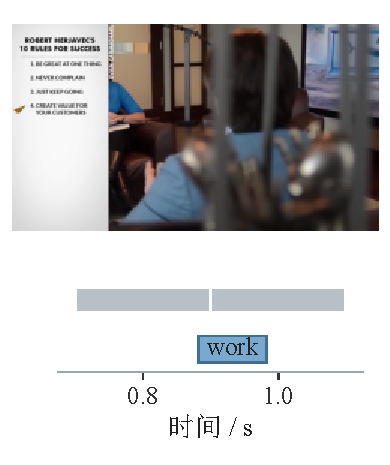
\includegraphics[width=\linewidth]{figures/fig_p1_observation_work.pdf}
        \caption{work的面部观测}
        \label{fig:p1_observation_work}
    \end{minipage}\hfill
    \begin{minipage}[t]{.32\linewidth}
        \vspace{0pt}
        \centering
        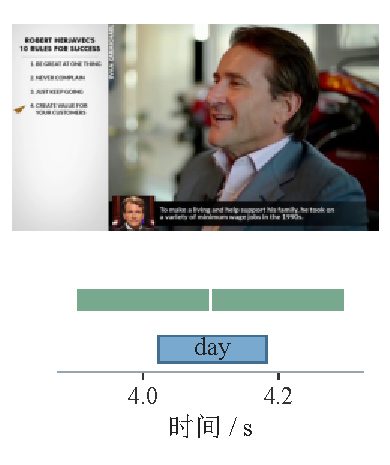
\includegraphics[width=\linewidth]{figures/fig_p1_observation_day.pdf}
        \caption{day的面部观测}
        \label{fig:p1_observation_day}
    \end{minipage}\hfill
    \begin{minipage}[t]{.32\linewidth}
        \vspace{0pt}
        \centering
        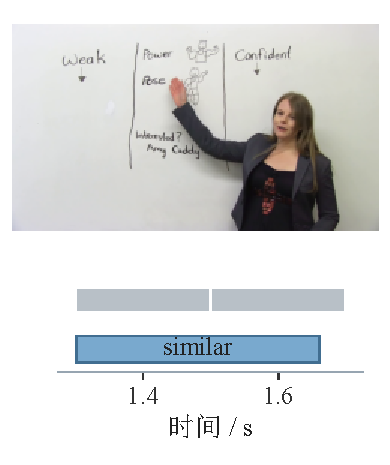
\includegraphics[width=\linewidth]{figures/fig_p1_observation_similar.pdf}
        \caption{similar的面部观测}
        \label{fig:p1_observation_similar}
    \end{minipage}
\end{figure}

\begin{figure}[htp!]
    \centering
    \begin{minipage}[t]{.48\linewidth}
        \vspace{0pt}
        \centering
        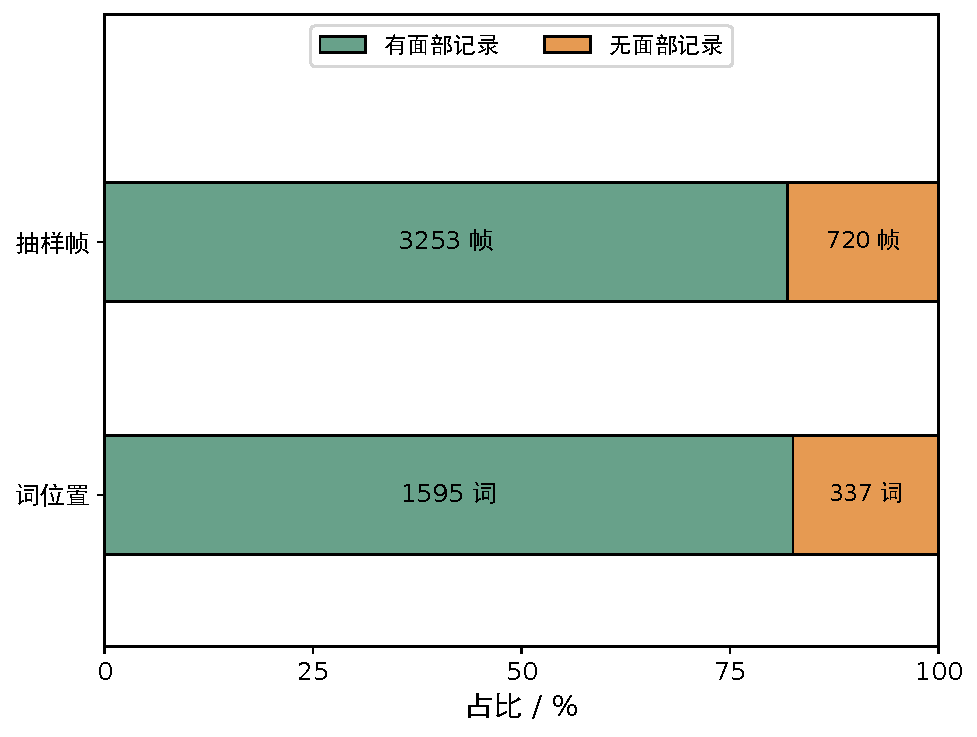
\includegraphics[width=\linewidth]{figures/fig_p1_visual_coverage.pdf}
        \caption{面部特征的帧级与词级覆盖}
        \label{fig:p1_visual_coverage}
    \end{minipage}\hfill
    \begin{minipage}[t]{.48\linewidth}
        \vspace{0pt}
        \centering
        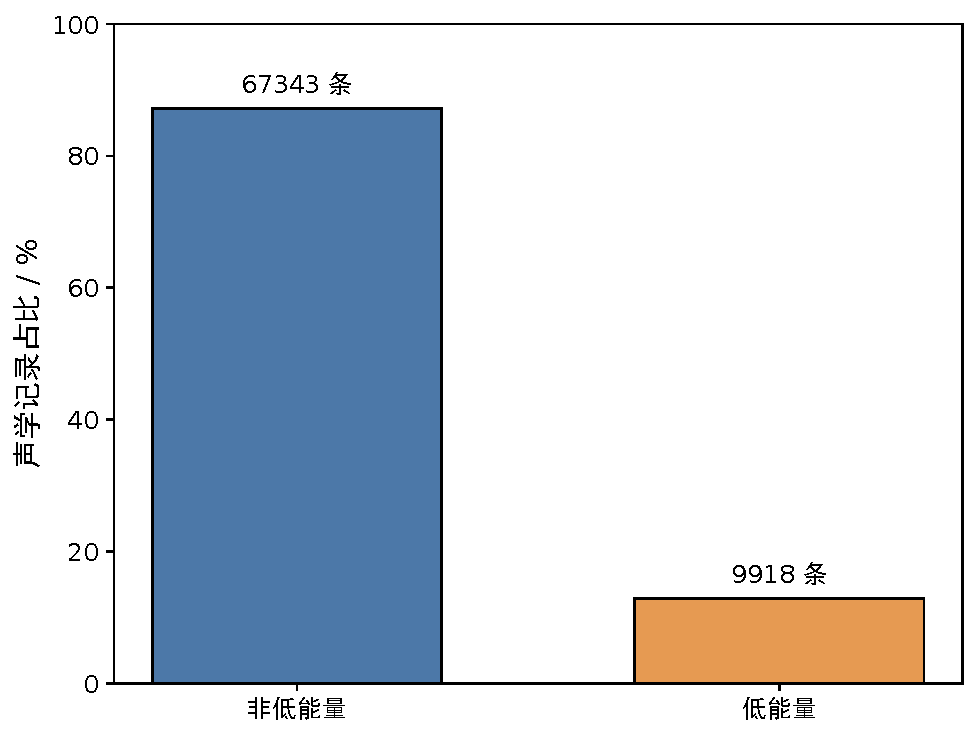
\includegraphics[width=\linewidth]{figures/fig_p1_audio_energy_share.pdf}
        \caption{声学记录的低能量占比}
        \label{fig:p1_audio_energy_share}
    \end{minipage}
\end{figure}

\begin{figure}[htp!]
    \centering
    \begin{minipage}[t]{.48\linewidth}
        \vspace{0pt}
        \centering
        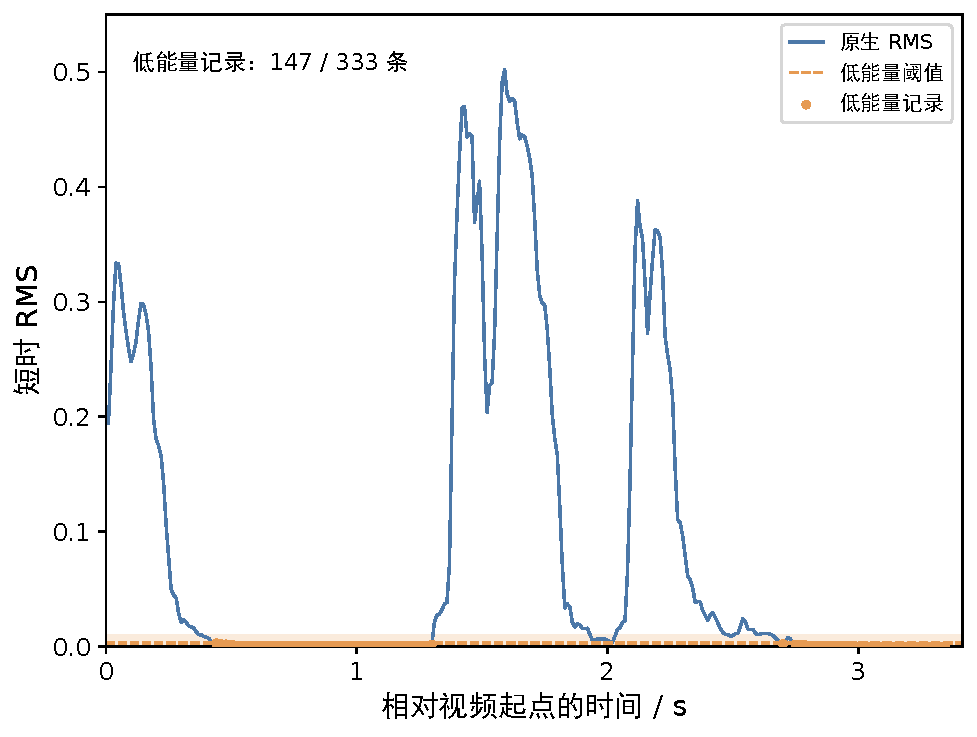
\includegraphics[width=\linewidth]{figures/fig_p1_rms.pdf}
        \caption{实例音频的短时RMS}
        \label{fig:p1_rms}
    \end{minipage}\hfill
    \begin{minipage}[t]{.48\linewidth}
        \vspace{0pt}
        \centering
        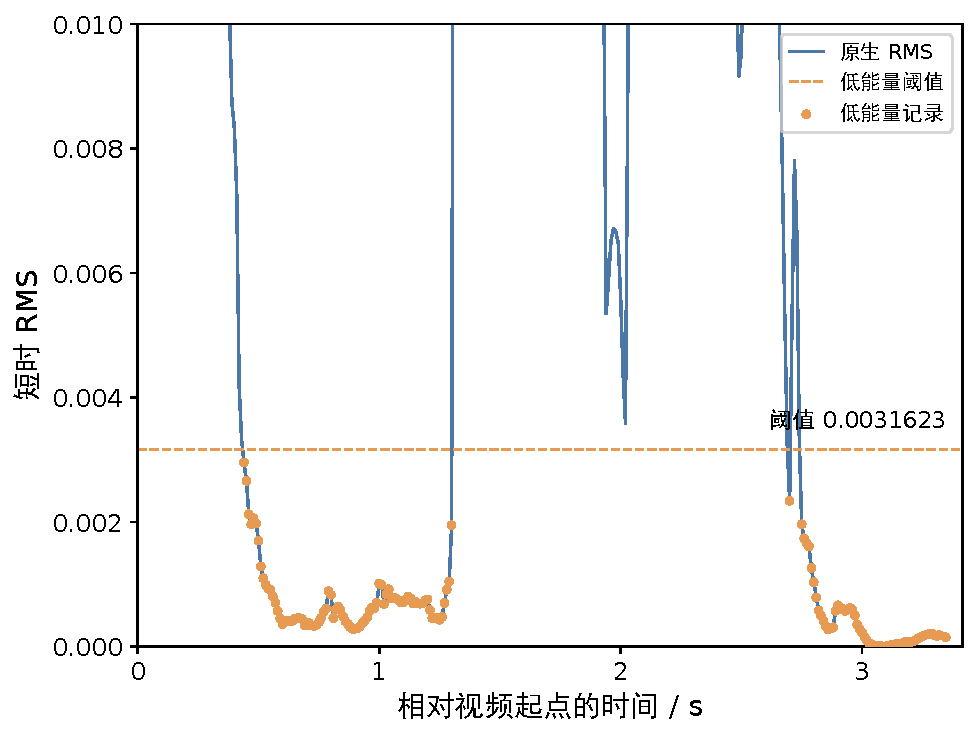
\includegraphics[width=\linewidth]{figures/fig_p1_rms_zoom.pdf}
        \caption{短时RMS的低幅值范围}
        \label{fig:p1_rms_zoom}
    \end{minipage}
\end{figure}

\begin{figure}[htp!]
    \centering
    \begin{minipage}[t]{.48\linewidth}
        \vspace{0pt}
        \centering
        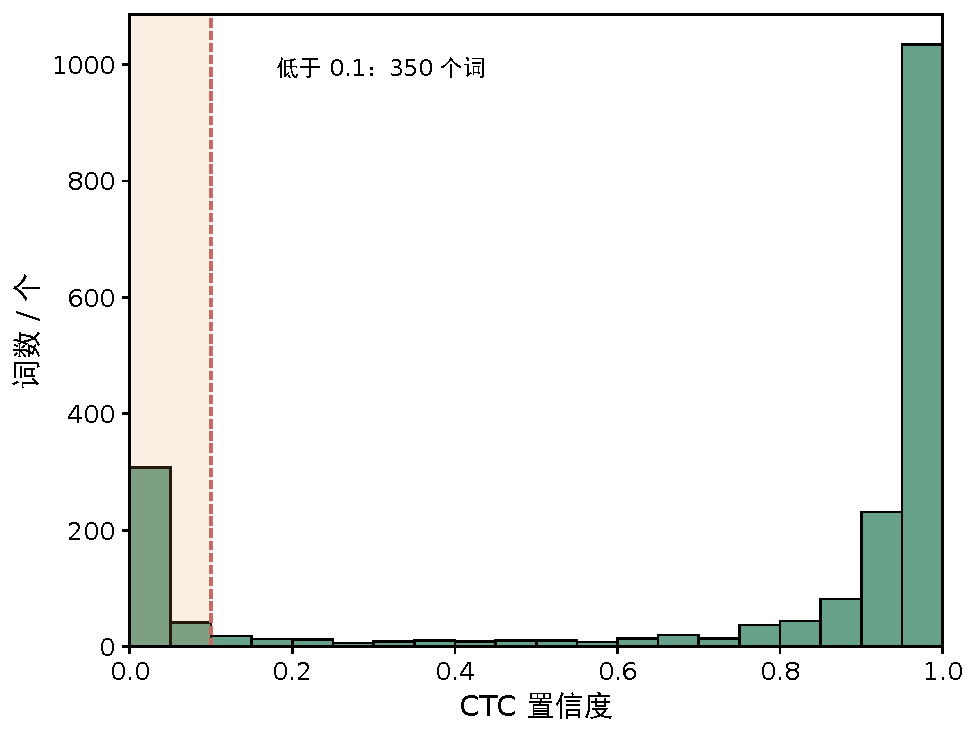
\includegraphics[width=\linewidth]{figures/fig_p1_ctc_confidence.pdf}
        \caption{词级CTC置信度分布}
        \label{fig:p1_ctc_confidence}
    \end{minipage}\hfill
    \begin{minipage}[t]{.48\linewidth}
        \vspace{0pt}
        \centering
        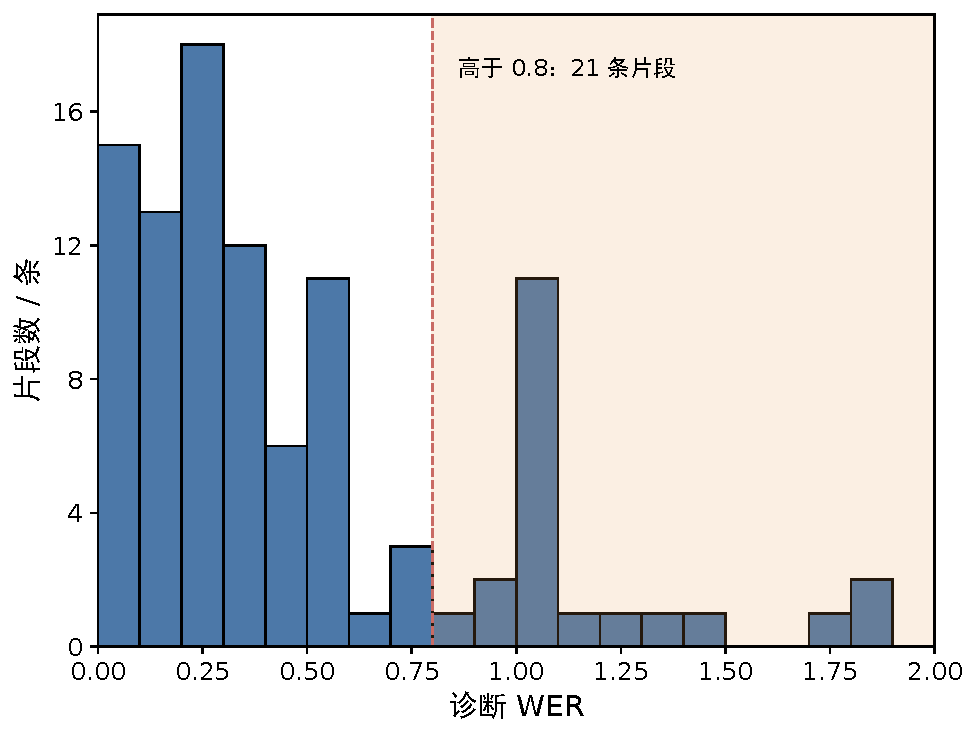
\includegraphics[width=\linewidth]{figures/fig_p1_diagnostic_wer.pdf}
        \caption{片段级诊断WER分布}
        \label{fig:p1_diagnostic_wer}
    \end{minipage}
\end{figure}

\begin{figure}[htp!]
    \centering
    \begin{minipage}[t]{.48\linewidth}
        \vspace{0pt}
        \centering
        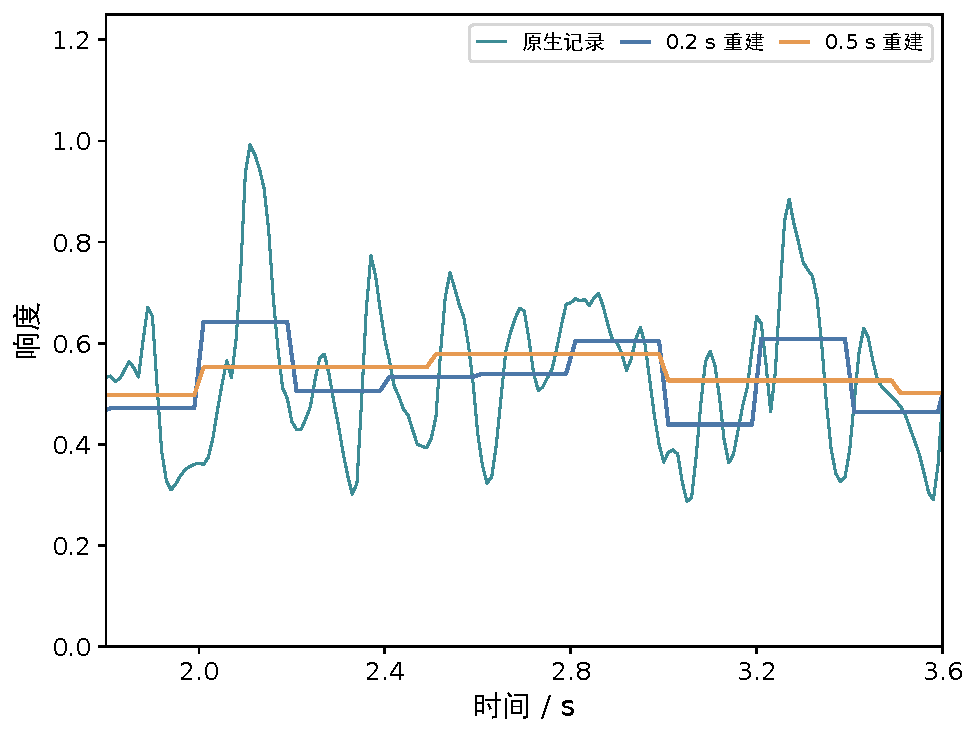
\includegraphics[width=\linewidth]{figures/fig_p1_window_reconstruction.pdf}
        \caption{响度的固定窗聚合与重建}
        \label{fig:p1_window_reconstruction}
    \end{minipage}\hfill
    \begin{minipage}[t]{.48\linewidth}
        \vspace{0pt}
        \centering
        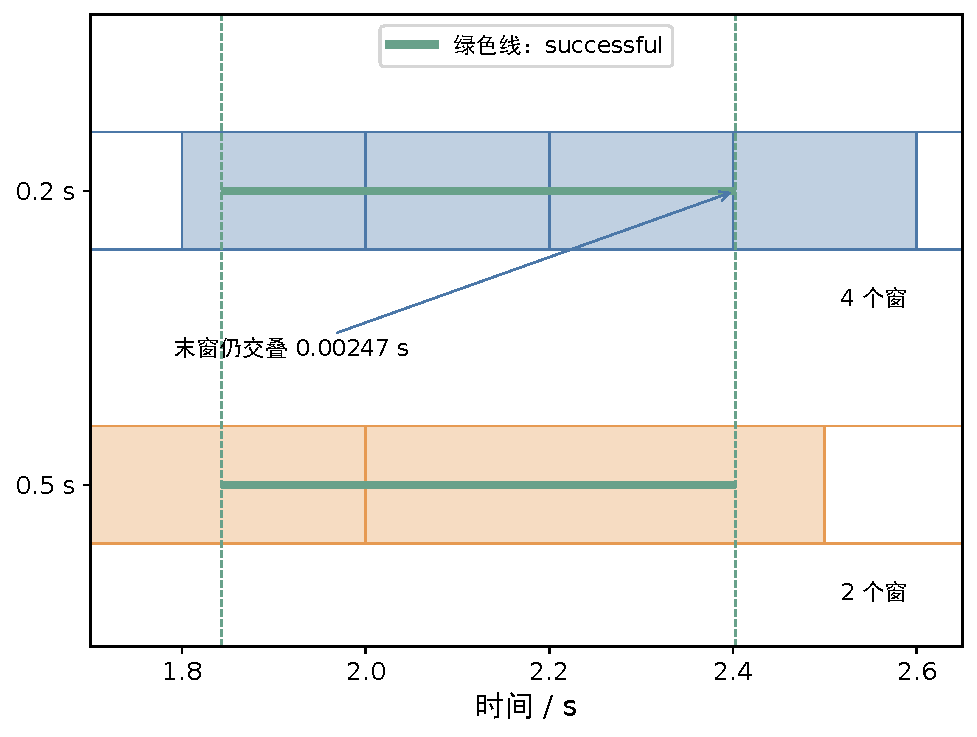
\includegraphics[width=\linewidth]{figures/fig_p1_word_window_overlap.pdf}
        \caption{候选词区间与固定窗口交叠}
        \label{fig:p1_word_window_overlap}
    \end{minipage}
\end{figure}

\begin{figure}[htp!]
    \centering
    \begin{minipage}[t]{.32\linewidth}
        \vspace{0pt}
        \centering
        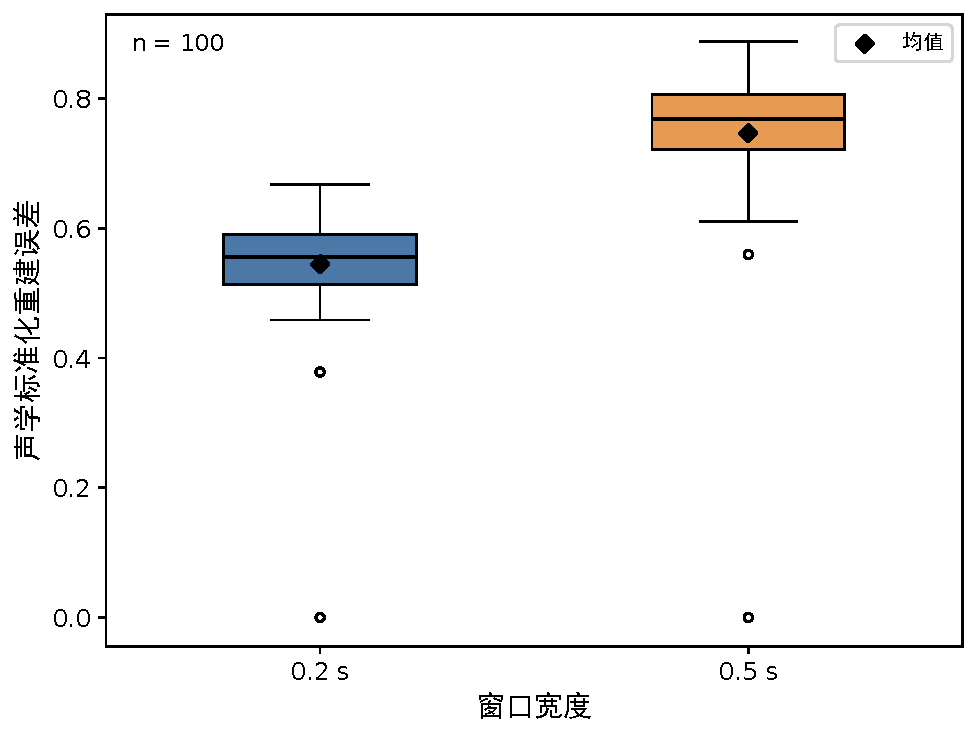
\includegraphics[width=\linewidth]{figures/fig_p1_audio_window_error.pdf}
        \caption{声学重建误差}
        \label{fig:p1_audio_window_error}
    \end{minipage}\hfill
    \begin{minipage}[t]{.32\linewidth}
        \vspace{0pt}
        \centering
        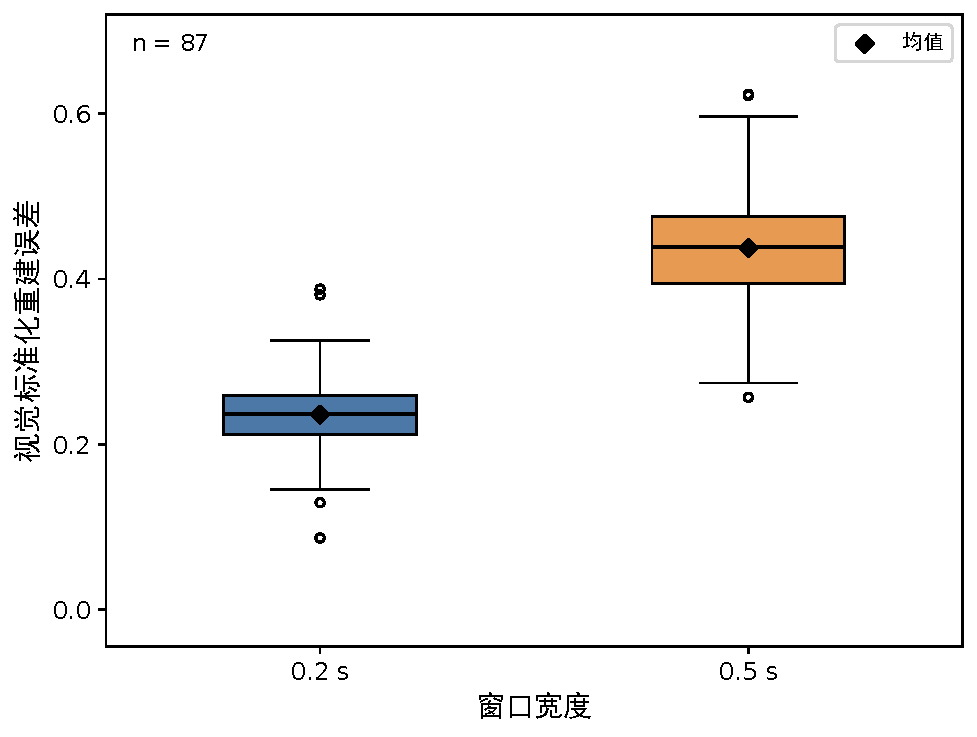
\includegraphics[width=\linewidth]{figures/fig_p1_vision_window_error.pdf}
        \caption{视觉重建误差}
        \label{fig:p1_vision_window_error}
    \end{minipage}\hfill
    \begin{minipage}[t]{.32\linewidth}
        \vspace{0pt}
        \centering
        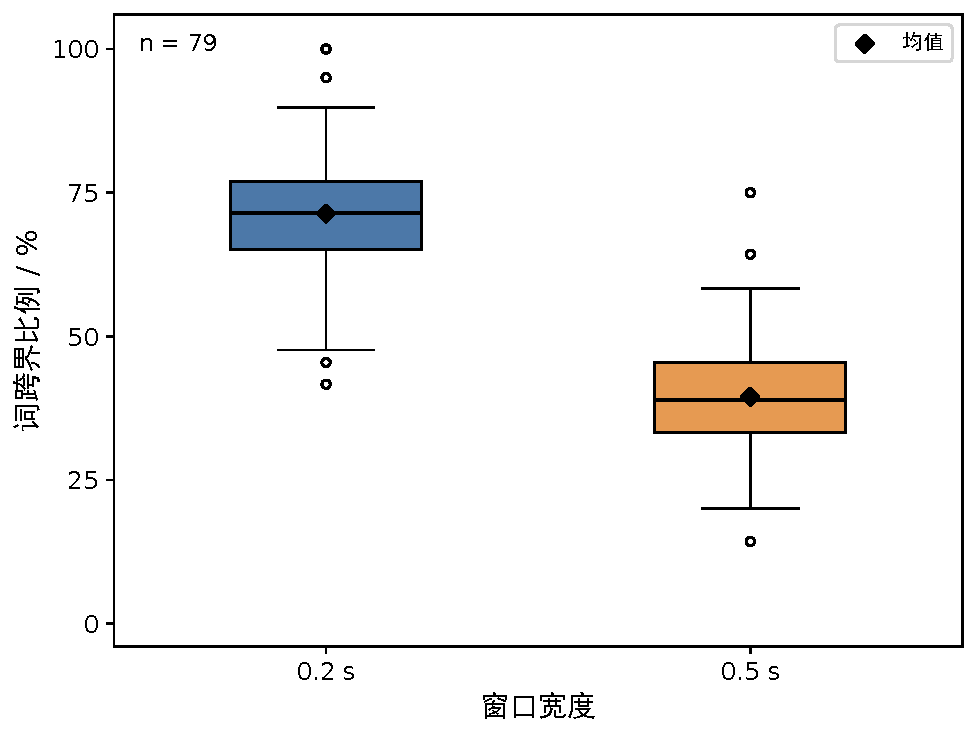
\includegraphics[width=\linewidth]{figures/fig_p1_word_crossing_ratio.pdf}
        \caption{词跨界比例}
        \label{fig:p1_word_crossing_ratio}
    \end{minipage}
\end{figure}

\begin{figure}[htp!]
    \centering
    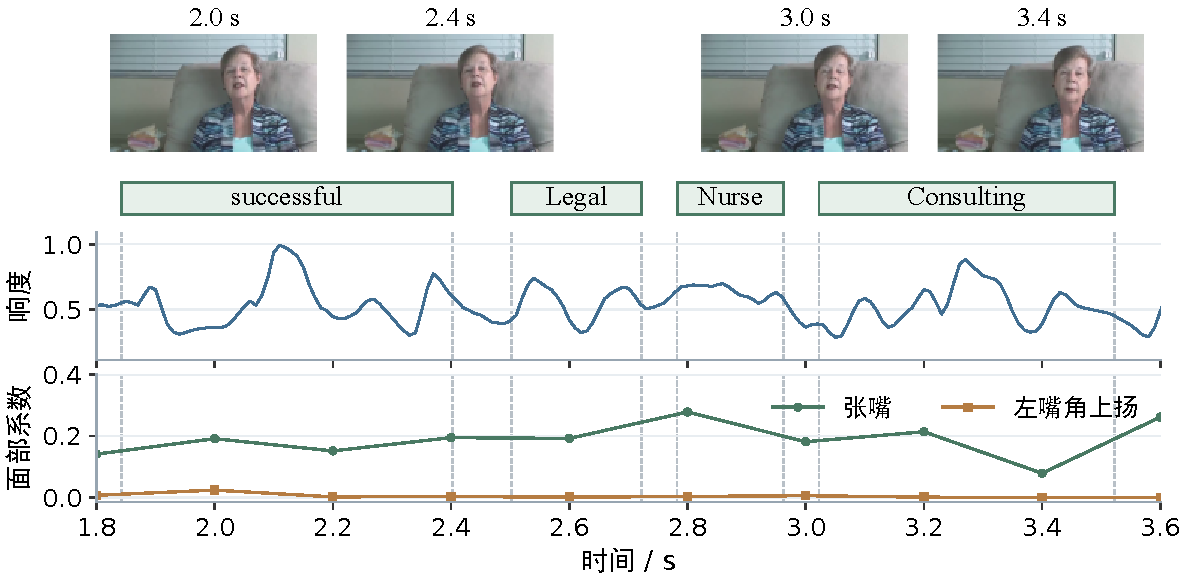
\includegraphics[width=0.94\linewidth]{figures/fig_p1_multimodal_timeline.pdf}
    \caption{典型样本的词区间与视听记录对应}
    \label{fig:p1_multimodal_result}
\end{figure}
